% !TEX root = ../ResearchBook.tex

\chapter{RFL with Facility Combinations: Reliable Sensor Deployment for Positioning/Surveillance via Trilateration}\label{chap:sensor}
\chaptermark{RFL with Facility Combinations: Sensor} % short chapter name

In this chapter, we incorporate the impacts of sensor disruptions into a reliable sensor deployment framework by extending the ideas of assigning backup sensors as well as correlation decomposition via supporting stations. 


\section{Introduction}\label{sensor:intro}

High-accuracy object positioning has been playing a critical role in various application contexts such as: (i) civilian uses, including vehicle navigation, driver guidance, activity tracking; (ii) industrial uses, such as aircraft tracking, regional surveillance, extrasolar planets detection; and (iii) military uses, such as search/rescue missions, missile and projectile guidance.

\begin{figure}[!htbp]
  \centering
    \subfigure[ideal case]{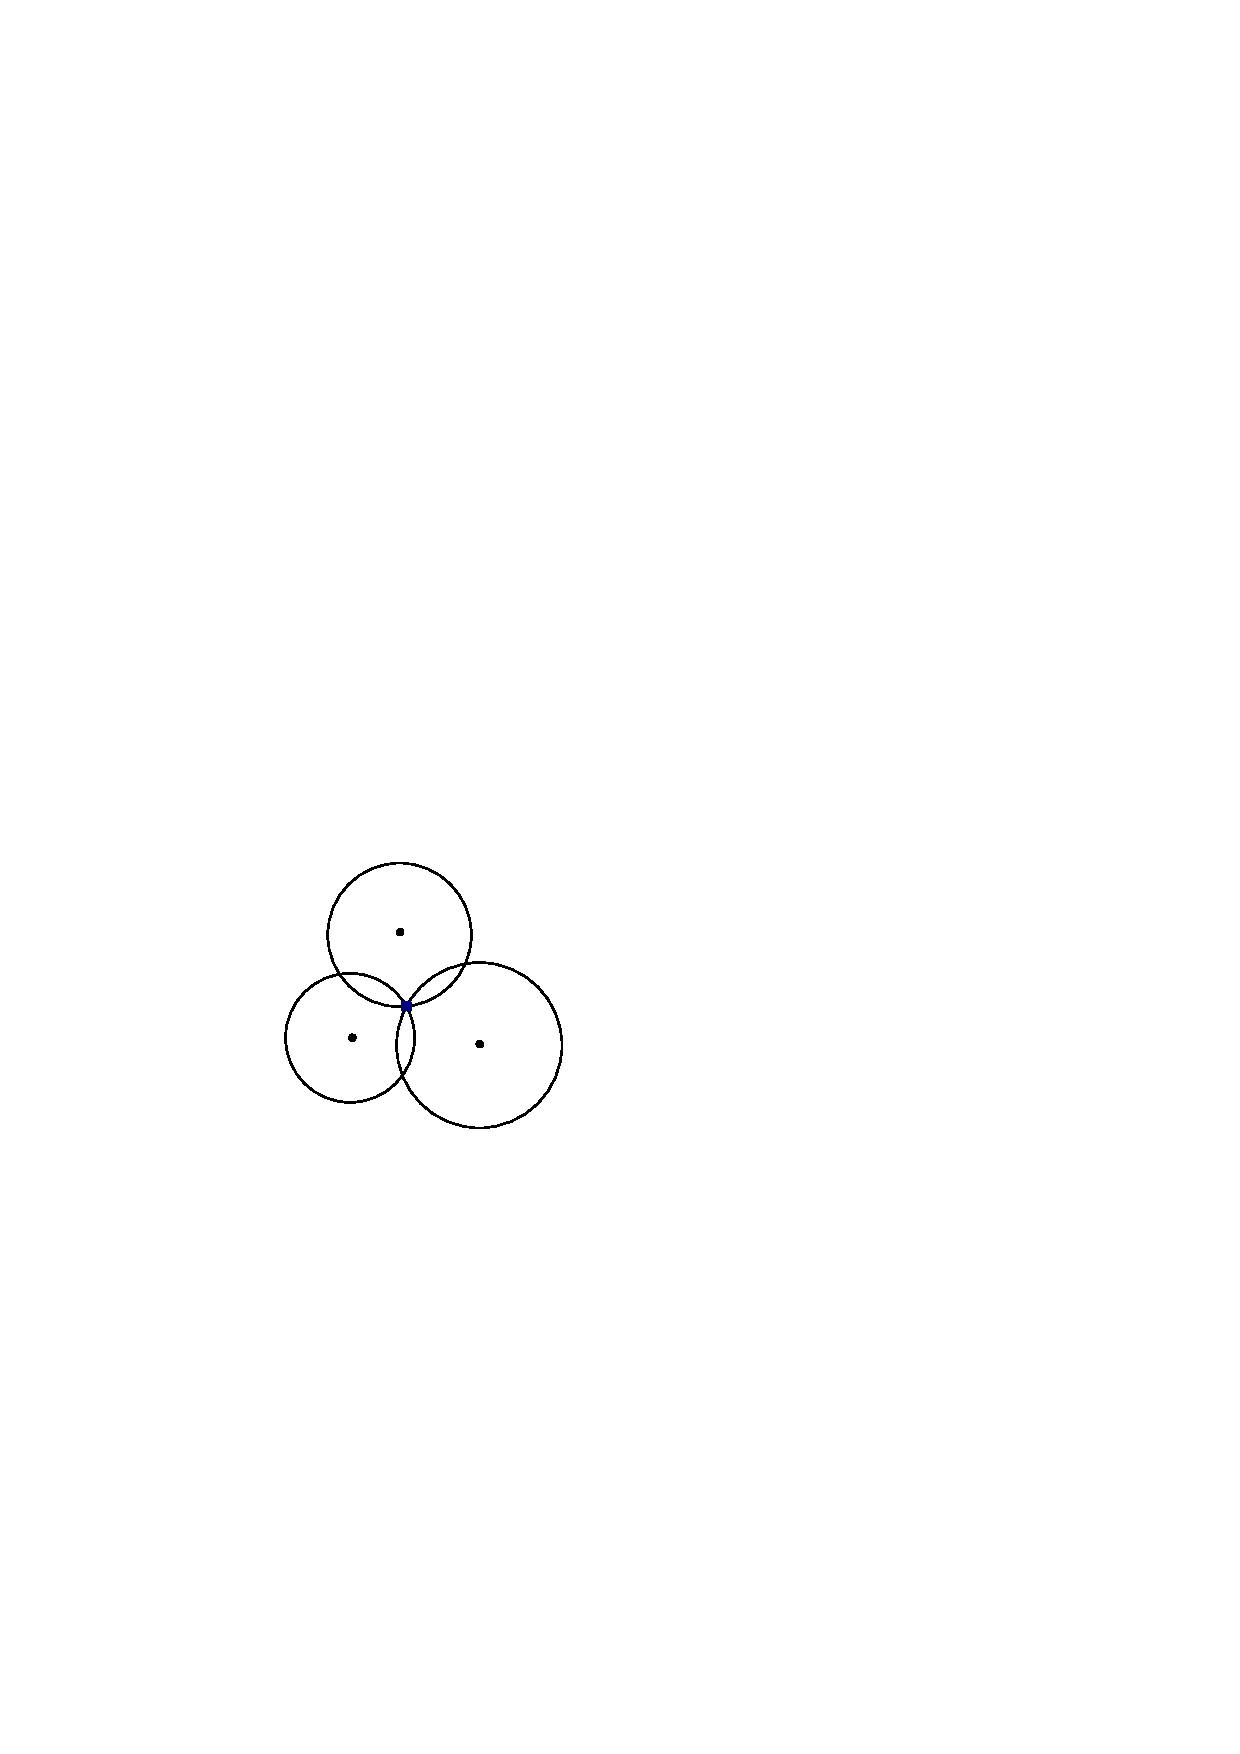
\includegraphics[width=0.19\textwidth]{images_sensor/1a.pdf} \label{fig:triletaration-a}} \hspace{5pt}
    \subfigure[three sensors]{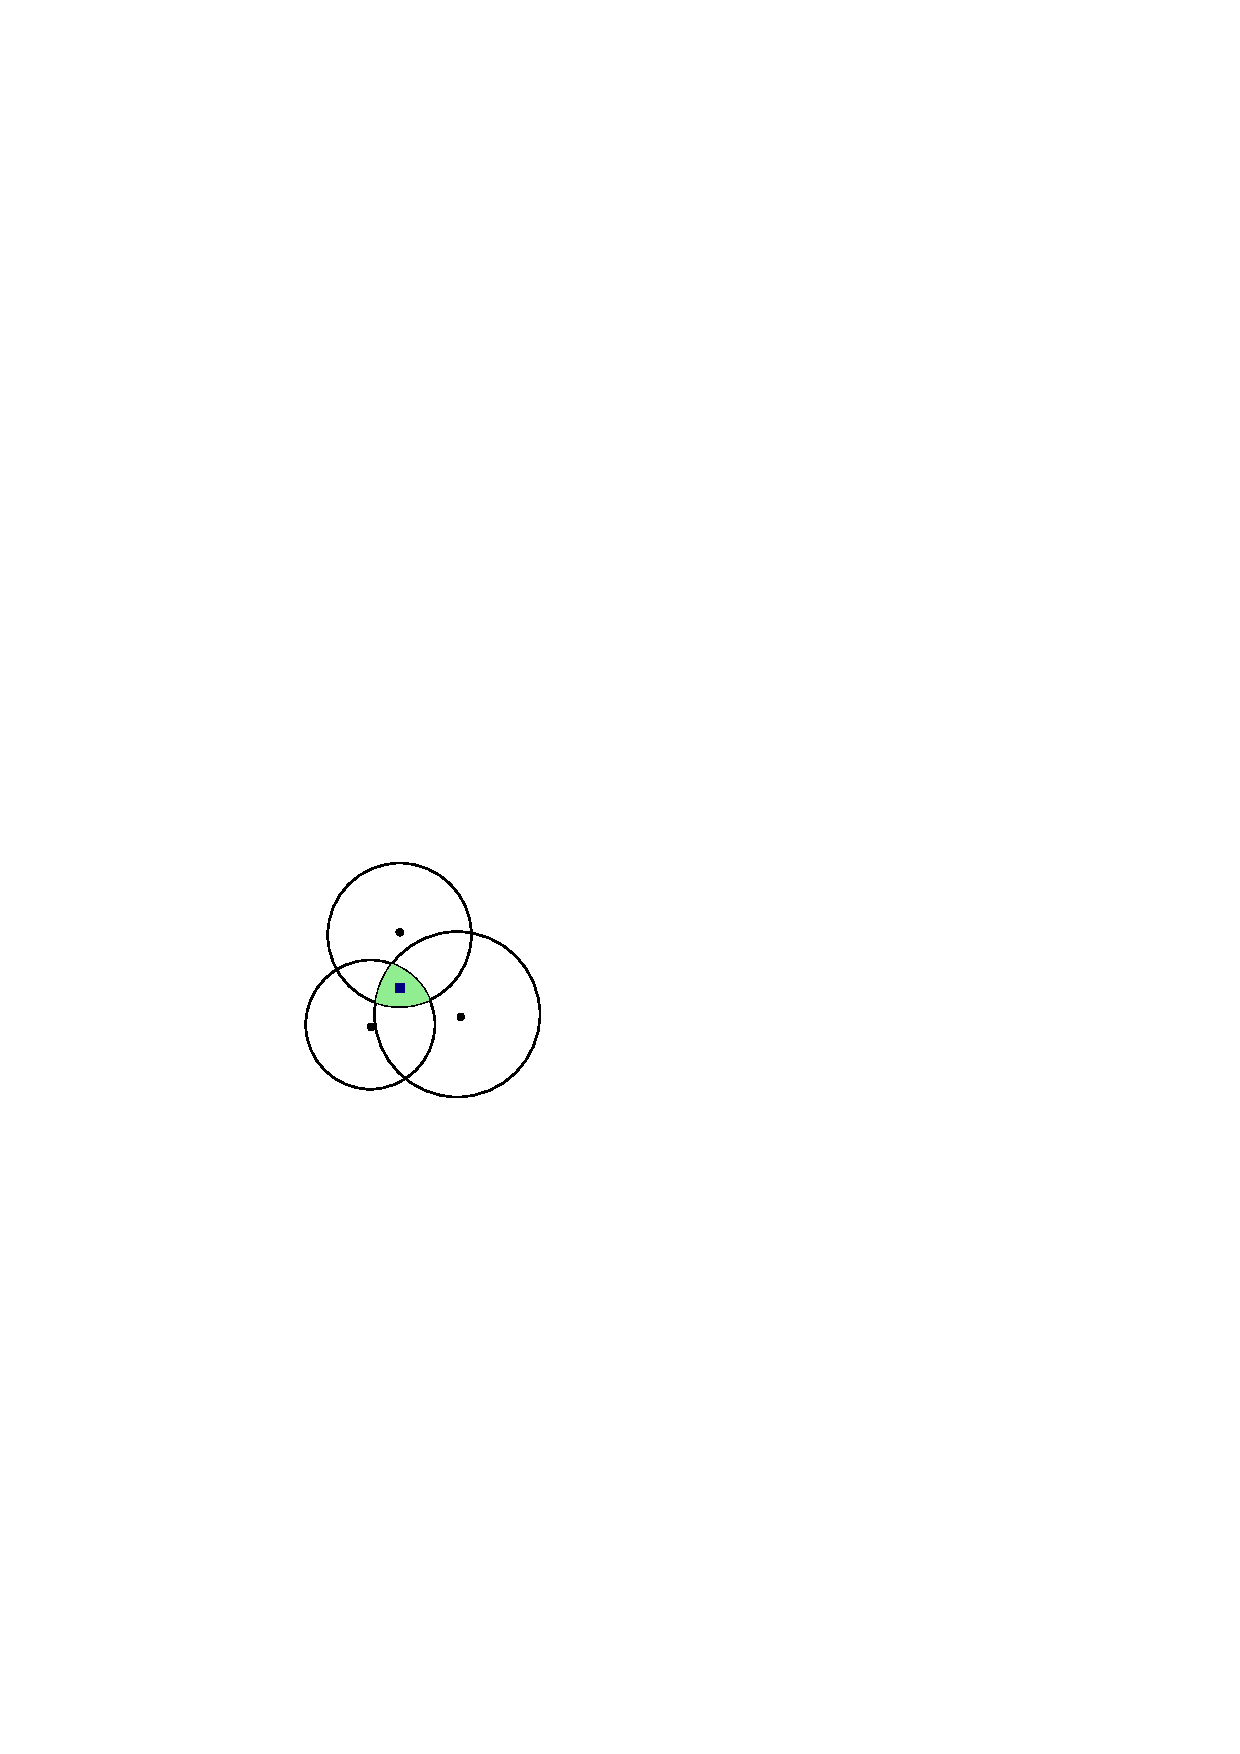
\includegraphics[width=0.19\textwidth]{images_sensor/1b.pdf} \label{fig:triletaration-b}} \hspace{5pt}
    \subfigure[multiple sensors]{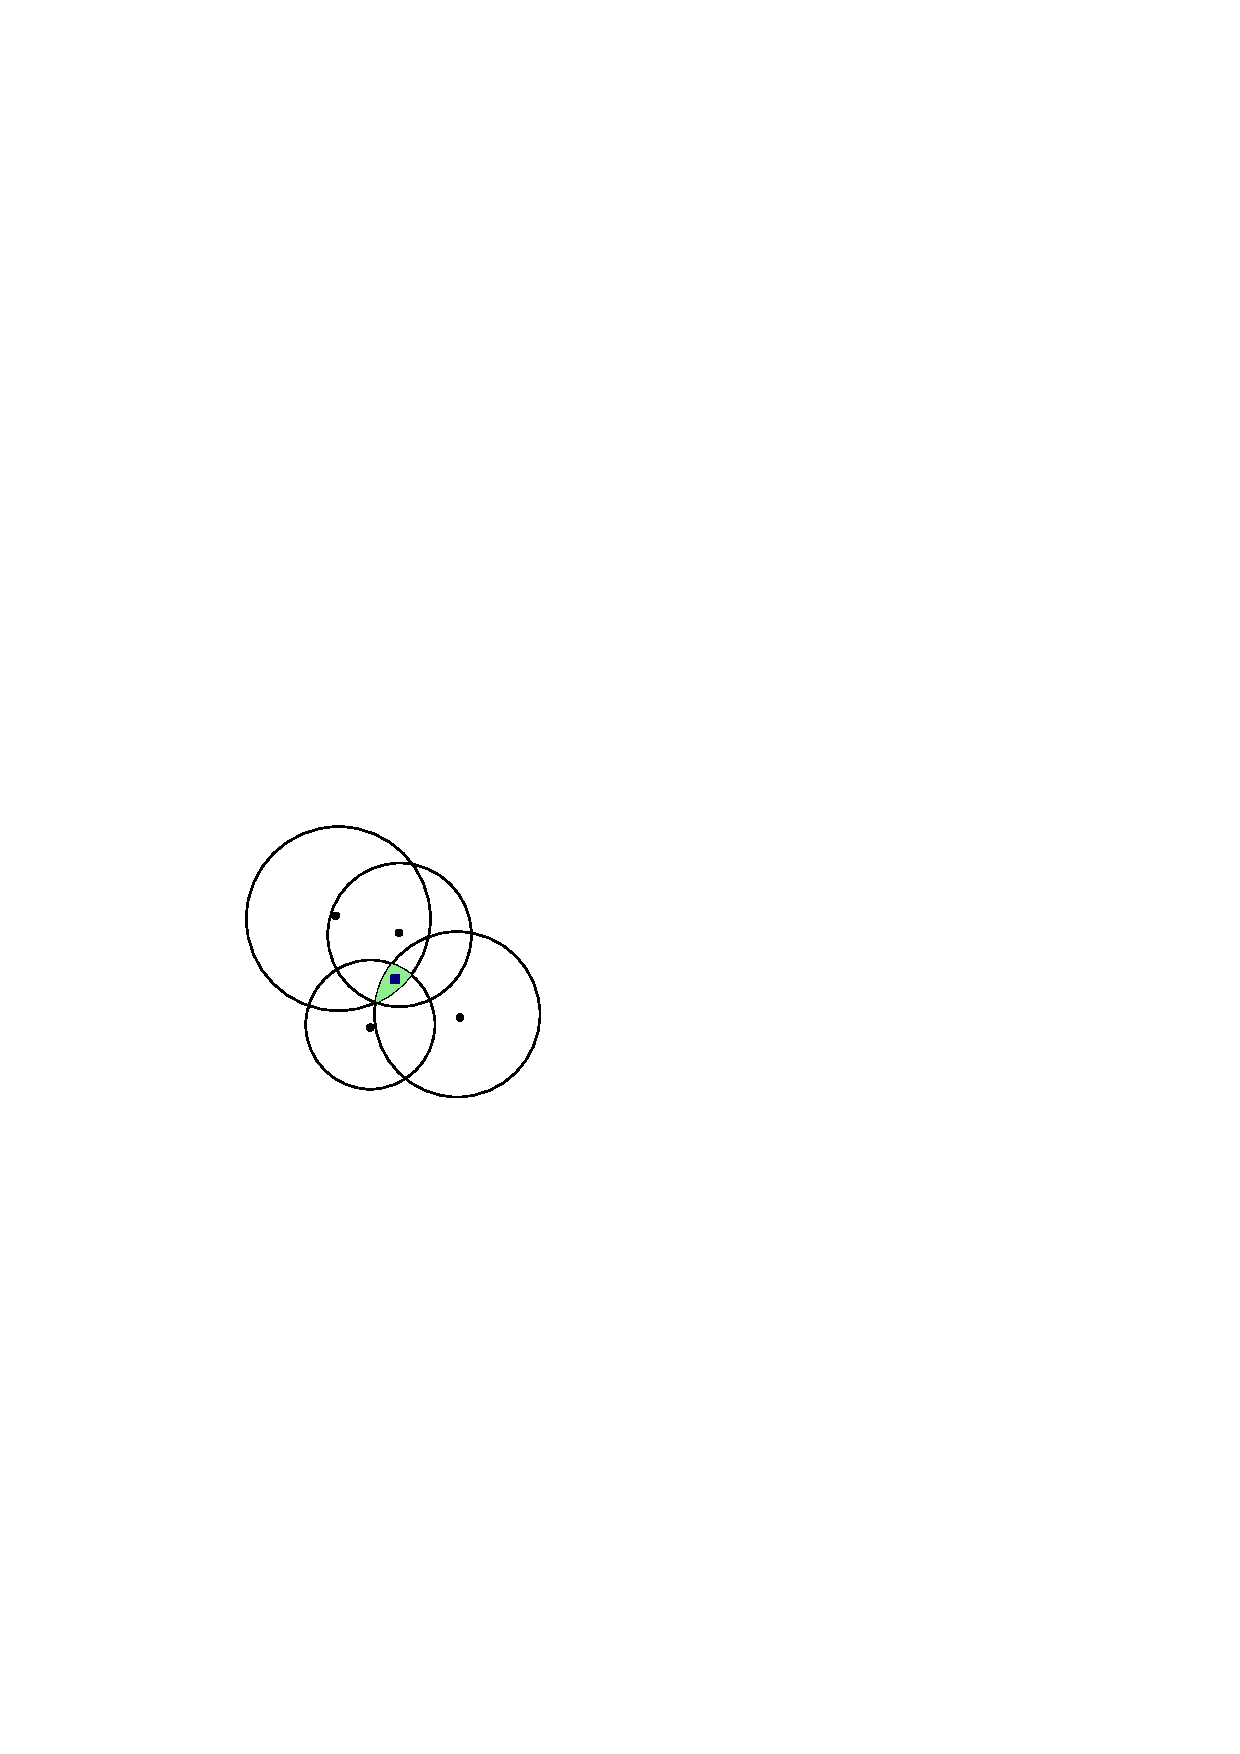
\includegraphics[width=0.19\textwidth]{images_sensor/1c.pdf} \label{fig:triletaration-c}} \hspace{5pt}
    \subfigure[disruption scenario]{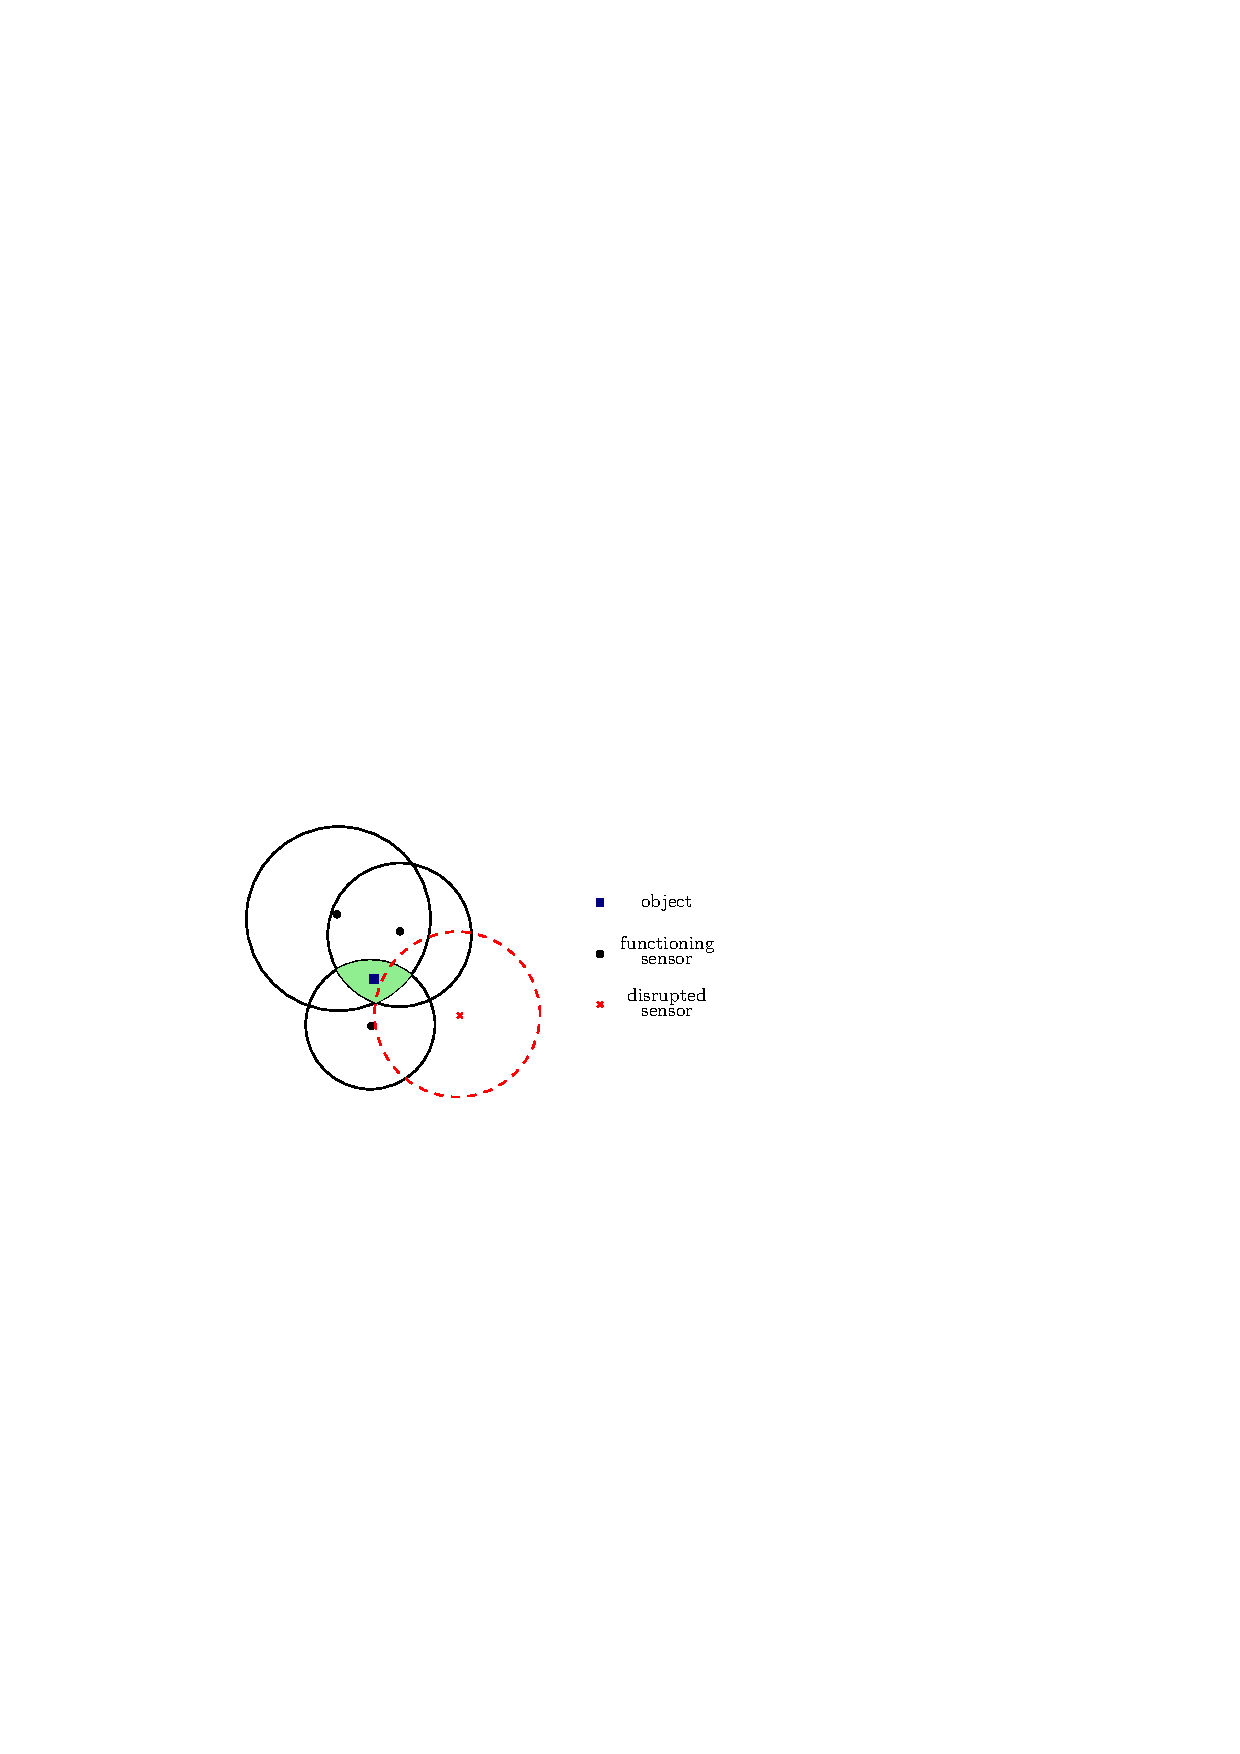
\includegraphics[width=0.32\textwidth]{images_sensor/1d.pdf} \label{fig:triletaration-d}}
  \caption{Position error illustration in trilateration.}
  \label{fig:illustration-trilateration}
\end{figure}

The remainder of this chapter is organized as follows. Section \ref{sensor:formulation} introduces the methodology we develop for the reliable sensor deployment problem, including the effectiveness measurements and the model formulation. Section \ref{sensor:algorithm} presents the solution algorithm. Section \ref{sensor:numerical} demonstrates the applicability of the model and solution algorithm on a series of examples.



\section{Model Formulation}\label{sensor:formulation}

This sensor location problem (SLP) can now be formulated as the following mixed-integer non-linear program:
\begin{subequations}
  \begin{align}
    (\text{SLP}) \quad \min_{\mathbf{X,Y,Z,P}} & \quad \sum_{j\in J} f_{j}X_{j} - \alpha\sum_{i\in I}\sum_{k\in K}\sum_{r=1}^{|\mathcal{J}|} v_{i}e_{ik}P_{ikr}Y_{ikr} \label{eqn:opt-a} \\
   \text{s.t.} & \quad \sum_{r=1}^{|\mathcal{J}|} Z_{ijr}\le X_{j}, ~\forall j\in J, i\in I, \label{eqn:opt-b} \\
   & \quad \sum_{r=1}^{|\mathcal{J}|} Z_{ijr}\le 1, ~\forall j\in J, i\in I, \label{eqn:opt-c}
  \end{align}
\end{subequations}


\begin{prop} 
  \label{prop:1}
    The assignment probability $P_{ikr}$ can be calculated recursively by \eqref{eqn:opt-b}.
\end{prop} 

\begin{proof}
  We substitute $P_{ikr-1}$ in the right hand side of \eqref{eqn:opt-c},
  \begin{align}
     P_{ikr} &= \frac{\prod_{j\in J}\left(1-p_{j}\right)^{a_{kj}}}{\prod_{j\in J}p_{j}^{a_{kj}}}\prod_{s\le r}\left[ \sum_{j\in \mathcal{J}} Z_{ijs}\left(p_{j}\right)^{1_{[j\in J]}} \right]. \label{eqn:2}
  \end{align}
  This completes the proof.
\end{proof}



\section{Solution Algorithm}\label{sensor:algorithm}
\subsection{Lagrangian Relaxation}\label{sensor:lagrangian}

\begin{theo}
In (LSLP), the sensor location variables $\mathbf{X}$ are correlated with the sensor level assignment variables $\mathbf{Z}$ by constraints \eqref{eqn:opt-b}.
\begin{subequations}
  \begin{align}
    (\text{RSLP}) \quad \min_{\mathbf{X,Y,Z,P}} & \quad \sum_{j\in J} (f_{j}-\sum_{i\in I}\mu_{ij})X_{j} \label{eqn:5-a} \\
    \text{s.t.} & \quad \eqref{eqn:opt-b} - \eqref{eqn:opt-c}. \nonumber
  \end{align}
\end{subequations}
\end{theo}

In this way, a very large portion of the district options is eliminated from the initial set. The pseudo-code for filtering the district options is summarized as Algorithm \ref{alg:districtgenerate}.

\begin{algorithm}
  \caption{Generate the set of feasible district options}
  \label{alg:districtgenerate}
  \vskip 0.5em
  \Algorithm{DistrictGeneration}()
  \begin{algorithmic}[1]
    \FOR{$i\in \mathcal{I}$}
      \STATE{sourceHeap$ \leftarrow$ createHeap($i$), stack$ \leftarrow \emptyset$, districts$ \leftarrow \emptyset$}
      \STATE{stack.push(DFSNode($i$, sourceHeap, districts))}
      \WHILE{stack is not empty}
        \STATE{node $\leftarrow$ stack.pop()}
        \IF{ $W_{\text{weight}}\cdot$ node.demand $\cdot(1-q) + W_{\text{compact}}\cdot$ node.compact $\le \overline{W}$}
          \IF{node.hash is in districts.hashList}
            \STATE{districts.setList.add(node.set), district.hashList.add(node.hash)}
          \ENDIF
        \ENDIF
      \ENDWHILE
      \STATE{remove $i$ from $\mathcal{G}$}
    \ENDFOR
  \end{algorithmic}
  \vskip 0.5em
  \hrule
  \vskip 0.5em
  \Algorithm{createHeap}($i$, visitedNodes)
  \begin{algorithmic}[1]
    \STATE{newHeap $\leftarrow \emptyset$}
    \FOR{$n\in \mathcal{E}(i)$}
      \IF{$n$ is not in visitedNodes}
        \STATE{newHeap.insert($n$)}
      \ENDIF
    \ENDFOR
    \RETURN{ newHeap}
  \end{algorithmic}
\end{algorithm}



\section{Numerical Examples}\label{sensor:numerical}

\subsection{Hypothetical Grid Networks} \label{sensor:hypothetical}

A 2$\times$3 rectangle grid network and six $n\times n$ square grid networks for $n\in\{3,4,5,6,7,8\}$ are generated to represent various hypothetical study regions. 

\begin{table}[htbp]
  \centering
  \footnotesize
  \caption{Algorithm performance comparison for the 7 hypothetical cases.}
    \begin{tabular}{cccccccc}
    \toprule
     & Sensor  & Neighborhood  & No. of   & Final  & Final  & Final     & CPU      \\
     & network & network       & sensors  & UB     & LB     & gap (\%)  & time (s) \\
    \midrule
    \multirow{5}[2]{*}{CPLEX} 
          & $2\times3$  & $1\times2$  & 2   & -1.31    & -1.30    & 0     & 1.6   \\
          & $3\times3$  & $2\times2$  & 4   & -14.01   & fail     & 100   & 3600  \\
          & $4\times4$  & $3\times3$  & -   & -        & -        & fail  & 3600  \\
          & $\cdots$    & $\cdots$    & -   & -        & -        & fail  & 3600  \\
          & $8\times8$  & $7\times7$  & -   & -        & -        & fail  & 3600  \\
    \midrule
    \multirow{7}[2]{*}{LR+B\&B}
          & $2\times3$  & $1\times2$  & 2   & -1.31    & -1.31    & 0     & 0.1   \\
          & $3\times3$  & $2\times2$  & 4   & -24.28   & -24.28   & 0     & 0.1   \\
          & $4\times4$  & $3\times3$  & 5   & -77.38   & -77.38   & 0     & 0.4   \\
          & $5\times5$  & $4\times4$  & 8   & -150.78  & -150.78  & 0     & 0.8   \\
          & $6\times6$  & $5\times5$  & 14  & -243.48  & -243.48  & 0     & 38    \\
          & $7\times7$  & $6\times6$  & 21  & -360.99  & -360.99  & 0     & 181   \\
          & $8\times8$  & $7\times7$  & 29  & -489.07  & -500.41  & 2.32  & 3600  \\
    \bottomrule
    \end{tabular}%
  \label{tab:sensor-casestudy-stat}%
\end{table}%
